\subsection{Utilisation et intérêt de l'apprentissage statistique - Deep Learning }

Dans cette partie, nous allons intéresser aux différentes motivations qui nous ont poussé à utilisé l'apprentissage statistique (ou Deep Learning) dans notre contrôleur. Dans notre introduction, nous avons énoncé quelques points qui nous ont influencé pour choisir cette technologique. Nous préciserons en quoi le Deep Learning est pertinent dans notre contexte et introduirons ses principaux concepts et comment l'incorporer avec l'apprentissage par renforcement.

\subsubsection{Motivation et objectif de l'apprentissage statistique}

Nous avons en introduction énoncé les principales contraintes qui reposées sur notre asservissement. De façon synthétique, nous avions trouvé:
\begin{itemize}
\item Environnement partiellement observable (possiblement bruité)
\item Agent doit être capable à partir d'un apprentissage sur une environnement d'être capable de réussir sur un environnement assez proche (généralisation)
\item Les entrées seront basées sur la vision de l'agent
\end{itemize}

Nous verrons que ces problématiques sont abordés par l'apprentissage statistique. La force du deep learning réside dans ça capacité à extraire de l'information à partir d'entrées bruitées à hautes dimensions. Néanmoins, le deep learning possède son lot de restriction parmi lesquels: 

\begin{itemize}
\item Cela nécessite de très nombreux exemples pour réussir son apprentissage.\\nous verrons qu'en RL il faudra parfois plus de $80*10^6$ d'images pour finir un apprentissage)
\item L'apprentissage est difficile et parfois non stable\\nous approfondirons ce point plus tard, mais il est à noter que selon l'architecture choisit et nos fonctions de pertes, la stabilité du réseau n'est pas garanti. De façon plus claire, il y a énormément de facteurs jouant sur la stabilité du réseau et il peut être difficile de régler ces facteurs pour obtenir de bon résultat. 
\item Le réseau peut sur apprendre (apprentissage par coeur des résultats) impliquant l'impossibilité de généraliser.
\end{itemize}

Malgré les difficultés énoncées, le deep learning rend possible notre contrôle basé sur la vision en temps réel d'un agent. 

Définissons le contexte dans lequel le deep learning s'inscrit. A chaque pas de temps, l'agent va recevoir l'image partielle de l'environnement (soit un tableau de pixels). Nous souhaitons en sortie avoir la probabilité d'actions selon l'état (soit la politique pour l'état rencontré).

\begin{center}

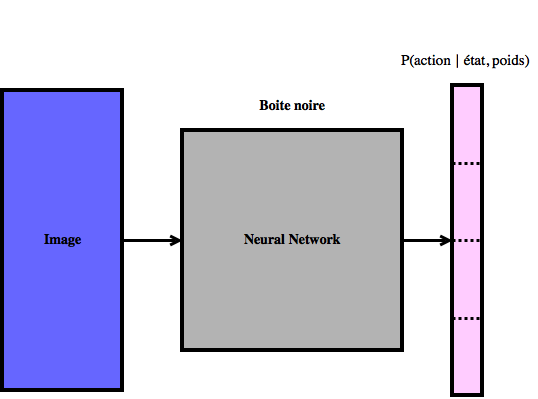
\includegraphics[width=.4\linewidth]{./assets/DeepLearning/dl}
\captionof{figure}{Représentation haut niveau de l'architecture classique en deep learning}
\end{center}

Bien évidemment, le deep learning peut être utiliser pour bien d'autre chose mais nous nous restreindrons à son utilisation dans le cadre de l'apprentissage par renforcement. Néanmoins la figure ci dessus reste d'actualité dans la cadre d'un apprentissage supervisé (exemple en classification: déterminer le nombre représenté par une image correspondrait à avoir en sortie du réseau $P(\text{nombre} \:\vert\: \text{état}, \text{poids)}$. 

Un problème est maintenant de définir comment va être générer  $P(\text{action } \:\vert\: \text{ état}, \text{poids)}$ et c'est là qu'apparait la véritable force du deep learning. On peut façonner automatiquement les poids du réseau de neurone dans le but d'optimiser une fonction de perte (ou de gain).

\begin{center}
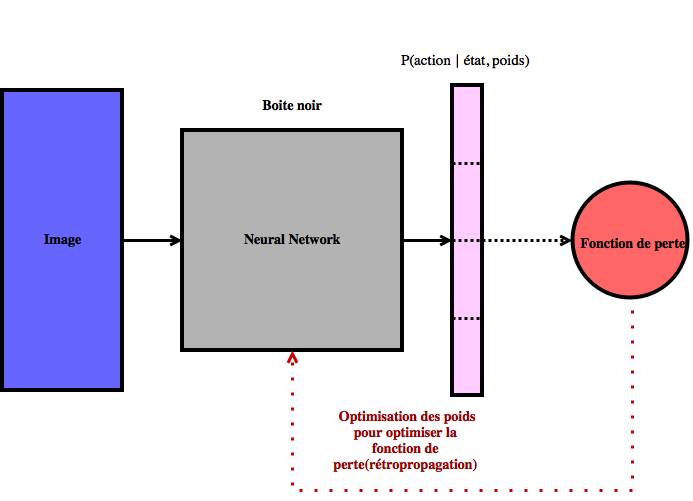
\includegraphics[width=.55\linewidth]{./assets/DeepLearning/dl2}
\captionof{figure}{Représentation haut niveau de l'architecture classique en deep learning avec optimisation de la fonction de perte}
\end{center}

Dans la partie suivante, nous expliquerons les mécanismes responsables de l'optimisation du de la fonction de perte pour véritable  définir ce que veut dire un apprentissage dans le contexte du deep learning. Nous commencerons par introduire ce qu'est un réseau de neurone dans sa forme la plus simple et nous expliquerons succinctement les évolutions utilisées (qui sont le réseau de neurone à convolution et les réseaux récurrents).

\subsubsection{Architecture en apprentissage statistique et réseau de neurone linéaire}

Nous allons commencer par expliquer la structure sur laquelle se base les réseaux de neurones (du moins historiquement) avec \emph{le modèle du perceptron}. 

On définira un ensemble de poids $w$ sous la forme d'un vecteur de poid $W$, l'entrée sera un vecteur $X$ de même dimension que les poids. On appelle $f$ la fonction d'activation qui est une fonction de $\mathbb{R}$ dans $\mathbb{R}$. La fonction d'activation est un hyperparamètre, c'est à dire que c'est à l'expérimentateur de la définir, on retrouve néanmoins quelques fonctions d'activations très utilisées, nous reviendrons sur l'intérêt des fonctions d'activations un peu plus tard. Dans le cas du perceptron, nous utiliserons la fonction d'activation $f(x) = \left \{
  \begin{tabular}{cc}
  +1 \text{si} W^TX > \theta &  \\
  -1 &  
  \end{tabular}
$

\begin{center}
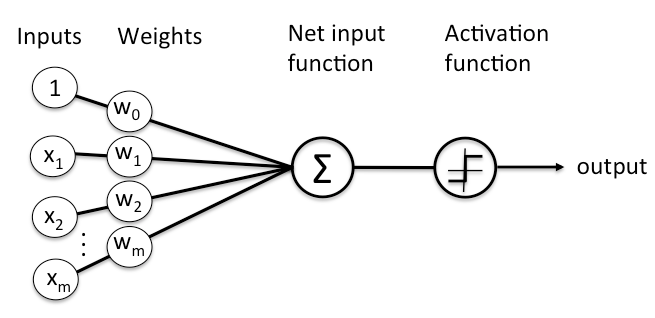
\includegraphics[width=.55\linewidth]{./assets/DeepLearning/perceptron_node}
\captionof{figure}{Représentation haut niveau de l'architecture classique en deep learning avec optimisation de la fonction de perte \cite{blogPerceptron}}
\end{center}


Pour se conformer à la figure 7, il nous reste à définir quelle est la fonction de coût et comment se passe le processus d'optimisation de la fonction de coût. Pour cela, nous avons encore besoin de quelques définitions. Plaçons dans un problème à deux classes (chien et chat par exemple) on définira la classe d'une entrée comme état la classe à laquelle l'entrée appartient ainsi on donnera $c(x) = \left \{
  \begin{tabular}{cc}
  1  \text{si} x \in \text{Chien}  &  \\
  -1 \text{si} x \in \text{Chat}&  
  \end{tabular}
$, cela nous permet donc de définir la façon dont on va optimiser les poids: 
$$ W_{t+1} = W_t - \alpha \big( c(x) - f(x) \big) x $$

\subsubsection{Réseau de neurones dense}
Dans cette partie, nous allons expliquer l'architecture de base utilisée dans le contrôle de l'agent.

Notre objectif est d'approximer une certaines fonction $y = f(x)$. Nous avons accès à un ensemble de entrées et sorties associées que l'on notera $\mathcal{D} = \bigg\{(x_1, y_1), ..., (x_N, y_N)\bigg\}$. Nous souhaitons déterminer la fonction $\overset{\sim}{f}_w$ tel que $\overset{\sim}{f}_w \sim f$, la fonction $\overset{\sim}{f}_w$ est défini comme $\overset{\sim}{f}_w(x) = Wx + b $. Nous pouvons alors de façon équivalent défnir notre objectif comme un problème d'optimisation où l'objectif est de minimiser l'erreur quadratique moyenne $E = \overset{N}{\underset{p=1}{\sum}}\:\big( \overset{\sim}{f}(x) - f(x) \big)^2$. Nous pouvons dès lors changer les poids dans le but de minimiser cette erreur (ou fonction de perte). La difficulté est que nous souhaitons être capable de \emph{généraliser}, c'est à dire que si nous prenons un nouvelle ensemble $X = \big\{x'_1, ..., x'_P \big\}$, nous souhaitons que notre fonction $\overset{\sim}{f}_w$ soit toujours aussi proche de $f$. Un problème en apprentissage statistique qui peut survenir est que le réseau ait appris l'ensemble $\mathcal{D}$ mais que l'approximation soit mauvaise dès lors que l'on présente un ensemble d'entrée non vu durant l'entrainement. De nombreuses stratégies ont été mise en place pour éviter ce problème.

Pourtant, en l'état nous sommes incapables d'approximer des fonctions non linéaire. Or notre souhait est d'utiliser un réseau de neurone pour approximer la fonction qui associe des états à l'action optimale pour obtenir le maximum de récompenses, on peut conjoncturer la non linéarité de cette fonction.

Pour parvenir à approximer des fonctions non linéaire, nous allons donc empiler des réseaux denses suivies de fonction non linéaire (appelées \emph{fonction d'activation}). En pratique, on utilisera les fonctions tangeant hyperbolique, sigmoide, relu ...

\begin{figure}[ht]
\begin{center}
    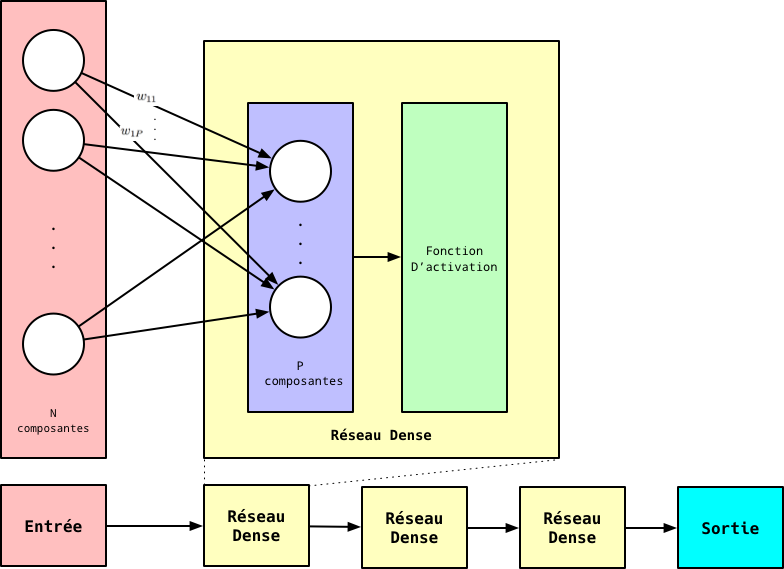
\includegraphics[scale=.3]{./assets/DeepLearning/Dense}
    \caption{Schéma d'un modèle dense et de la réalisation d'un réseau dense}
\end{center}
\end{figure}
En notant: $g^l$ pour la l ième fonction d'activation, la formule donnant la dynamique du l-ième module est: $$h^{(l)} = g^{(l)}\big(W^{(l)}h^{(l-1)} + b^{(l)} \big)$$
Les réseaux denses bien qu'extrêmment utile ont deux défaults majeurs. Le premier est l'incapcité des réseau de neurones denses à prendre en compte la temporalité. Or, dans notre cas, les actions précédent sont importantes pour déterminer l'action à effectuer. Deuxièmement, les réseaux denses ne sont pas les plus adaptés pour des tableaux de pixels (images) en entrée. Les réseaux de convolutions utilisent certaines spécificité du format image que n'utilise pas le réseau dense. Nous reviendrons sur les architectures palliant aux deux défauts cités précédemment. 

\subsubsection{Réseau de convolution et récurrent}
le réseaux de neurones à convolutions utilise l'opération de convolution pour déterminer la sortie du réseau. 
$$S(i,j) = (I * K) (i, j) = \underset{m}{\sum} \underset{n}{\sum} I(m,n) K(i-m, j-n)$$

Avec K le noyau et I l'entrée. On peut considérer l'opération de convolution comme une moyenne locale mouvante. Ainsi, elle permet d'être plus robuste aux bruits mais à de nombreux autres atouts.


Les réseaux de convolution utilisent en entrée des blocs de dimensions 3 (en pratique des tenseurs à 4 dimensions mais par simplicité, nous considerons simplement l'entrée comme un bloc 3D. On pourra penser une image RGB comme un bloc de dimension 3 dans laquelle la dernière dimension est composées des composantes bleu rouge vert). Le réseau de convolution s'est bati autour de trois idées. La première est des \textbf{intéractions locale}, ce qui veut dire que chaque entrée va intéragir avec seulement un sous ensemble de la sortie. La deuxième est le \textbf{partage des poids }, car dans le réseau a convolution, le noyau est commun à tout les pixels d'entrée (alors qu'on pourrait le changer pour chaque pixel). Cela a pour effet d'utiliser bien moins de paramètres qu'un réseau dense à taille équivalente. Enfin, troisièmment, le réseau possède \textbf{une invariance par translation}, cela implique que si un objet est translaté en sortie de réseau le résultat sera le même. Cela permet d'être plus robuste dans de nombreux cas.

Le réseau de convolution est composé d'un noyau qui est l'équivalent des poids dans le réseau de neurones denses. Il est utilisé dans l'opération de convolution. C'est le noyau qui est optimisé dans le but de minimiser une certaine fonction de coût.

\begin{figure}[h!]
\centering
\begin{minipage}{.5\textwidth}
  \centering
  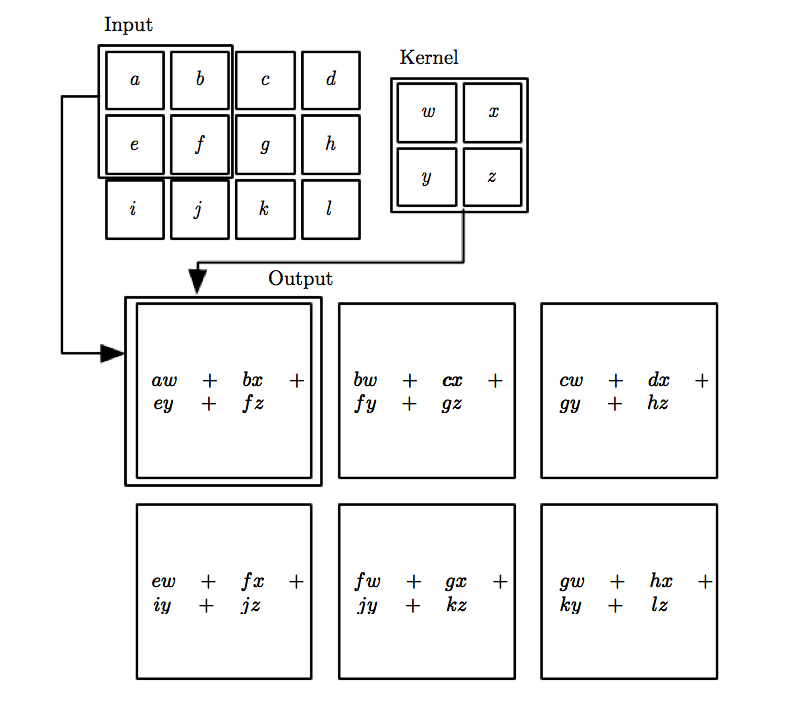
\includegraphics[width=.4\linewidth]{./assets/DeepLearning/conv.png}
  \caption{Opération de convolution dans un CNN}
\end{minipage}%
\begin{minipage}{.5\textwidth}
  \centering
  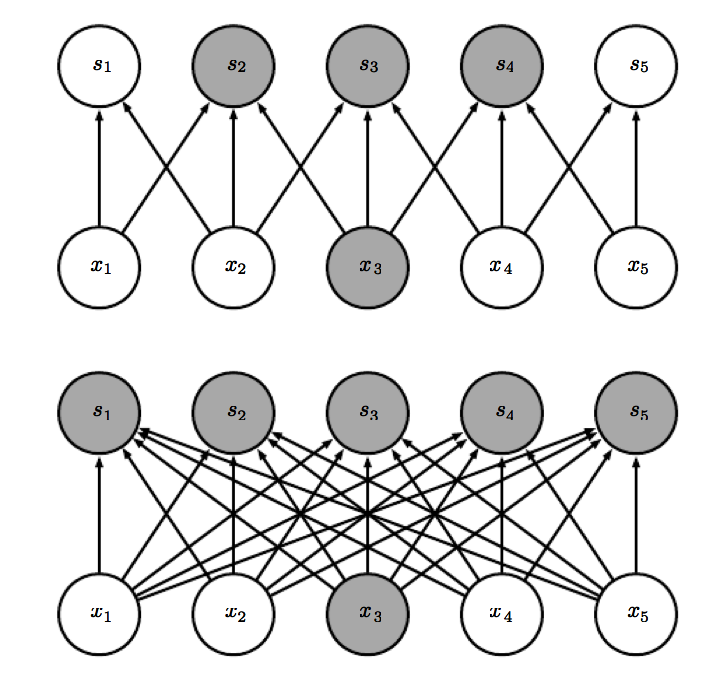
\includegraphics[width=.4\linewidth]{./assets/DeepLearning/convVSdense.png}
  \caption{Activation de  $x_3$} 
\end{minipage}
\end{figure}

Les réseaux de neurones récurrent ont été créé dans le but de pouvoir être utilisé avec des données séquentielles.
La dynamique d'un réseau récurrent est donnée pour un niveau L par la formule suivante:


\begin{gather*} 
    \left \{ \begin{tabular}{c}
            h_t = \tanh(W_{xh}x_t + W_{hh}h_{t-1} + b_h) &
            y_t = W_{hy}h_t + b_y &
    \end{tabular}
\end{gather*}

La formule ci dessous donne la dynamique du réseau récurrent le plus simple. Il souffre de nombreux problème, des alternatives existent notamment le réseau récurrent \emph{Long-Short term memory}\cite{LSTM}
. 

\begin{figure}[h!]
\begin{center}
    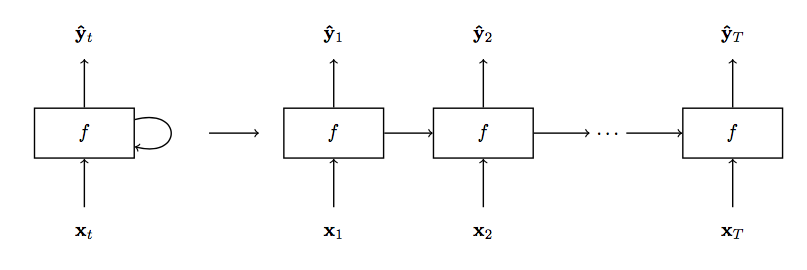
\includegraphics[scale=.5]{./assets/DeepLearning/reccurent.png}
\end{center}
\end{figure}

\subsubsection{Utilisation du deep learning dans le cadre de l'apprentissage par renforcement}

Dans la partie précédente, nous avons expliqué dans quel cadre il est pertinant d'utiliser l'apprentissage statistique (ou deep learning). Maintenant, nous allons comment intervient précisement cette technologie dans notre contrôle par apprentissage par renforcement. 

Comme nous l'avons vu, les principaux algorithmes d'apprentissage par renforcement utilise soit la fonction d'état (V), soit la fonction d'état action (Q). Ces fonctions sont une mesure de la qualité d'un état ou d'une action selon une politique. Ainsi, il joue un rôle  centrale dans le contrôle de notre agent. Plus encore, ces deux fonctions sont inconnus, et la réussite du contrôle de l'agent repose en grande partie sur notre capacité à approximer ces fonctions. Compte tenu de la complexité supposé de ces fonctions, nous avons décider d'utiliser l'apprentissage statistique car elle a montré sa capacité à apprendre des fonctions très complexe (non linéaire).

Dans la partie précédente, nous avons introduit l'apprentissage statistique supervisé (car non connaissons les sorties souhaitées). Or, dans notre cas nous serons dans un cas dit non supervisé car nous n'avons aucun signal sur lequel travaillé pour avoir la Q ou V fonction. Notre réseau devra approximer la fonction d'état avec un signal peu intéressant qui la récompense. Cela n'est pas suffisant, nous recherchons un réseau capable d'extraire d'un état qui lui est présenté les éléments qui sont suffisamment discrimant pour juger de la qualité d'une politique (via la V ou Q fonction).


Nous pouvons donc décomposer notre architecture d'apprentissage en deux partie. La première aura pour but d'extraire de l'état les élements importants pour caractériser la qualité de l'état (la V ou Q fonction). La deuxième aura pour but d'utiliser les éléments qui sont sortie de la première partie (soit des élements plus ou moins représentatif de la qualité) et devra les utiliser pour approximer la Q (ou V) fonction.


Voici une vue schématique de l'architecture réalisée dans le papier \emph{Human-level control through deep reinforcement learning}\cite{mnih-dqn-2015}
\begin{figure}
\begin{center}
    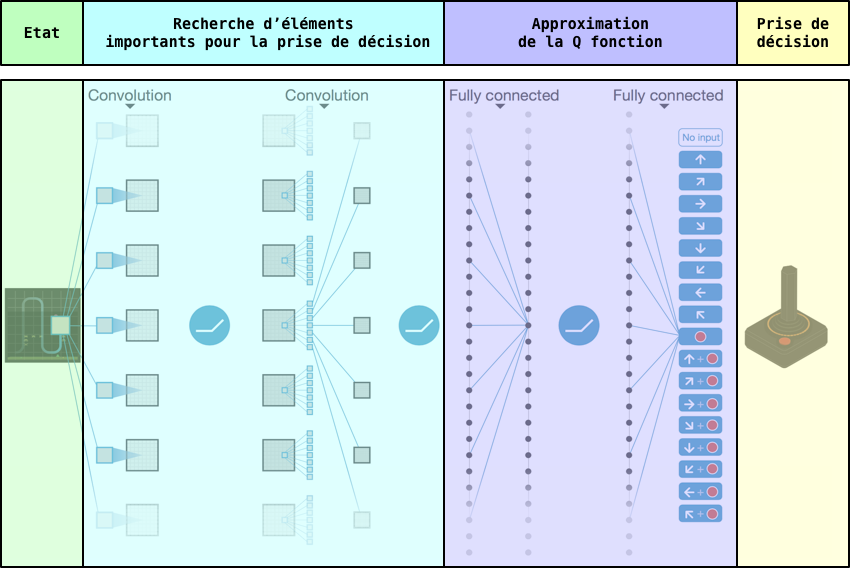
\includegraphics[scale=.5]{./assets/DeepLearning/DP_EX.png}
    \caption{Schéma récapitulatif des différentes sous parties dans un réseau de neurone utilisé pour de l'apprentissage par renforcement}
\end{center}
\end{figure}
